\subsection{Progettazione agli oggetti}\label{subsec:projagliobj}
Procediamo al raffinamento del modello di dominio continuando con la documentazione
dell'Architettura Software. Ora andremo a dettagliare le interazioni del sistema,
puntualizzando quali classi del modello del dominio risponderanno
alle procedure identificate nella fase precedente (v. Sezione 
\vref{sec:docarchsoft}).

Per effettuare quest'analisi, applicheremo il pattern \textit{Controller}, ovvero
ci chiediamo \textit{quale sia il primo oggetto, oltre allo strato UI} (indicato
genericamente nei nostri diagrammi tramite una generica classe non appartenente
al nostro Modello di Dominio \texttt{UIStrate}), \textit{a ricevere ed a coordinare un'operazione
di sistema}. In questa sede introdurremo anche le funzioni che saranno 
utilizzate allo scopo di effettuare le chiamate alla classe \texttt{DB}, allo scopo 
di interagire con il Database.
\subsubsection{Utente: Vista dei Casi d'Uso}


\begin{figure}[!thp]
 \centering
   \subfloat[][\emph{bindTutorForPatient}.]{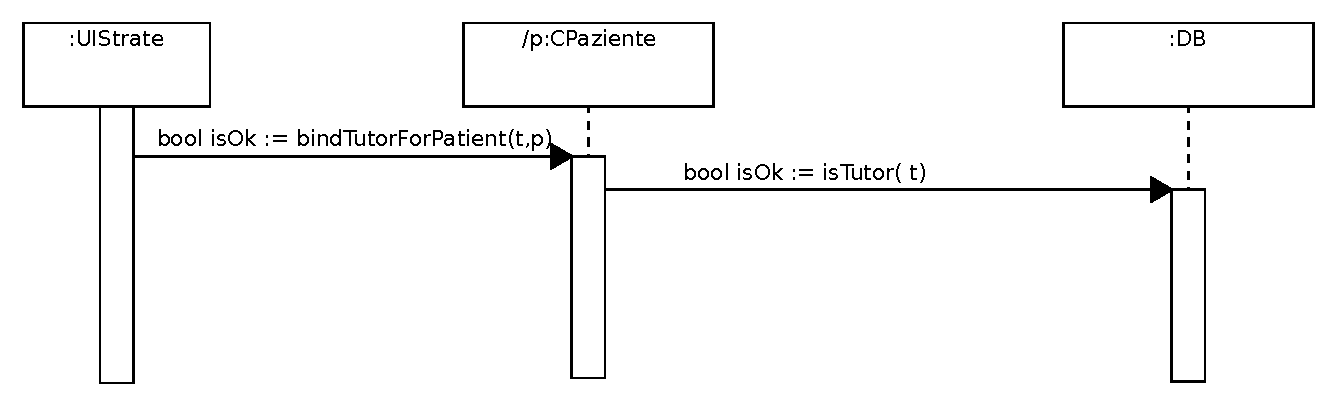
\includegraphics[scale=0.5]{svgs2/p_bindTutorForPatient}}\\
   \subfloat[][\emph{deferReservation}.]{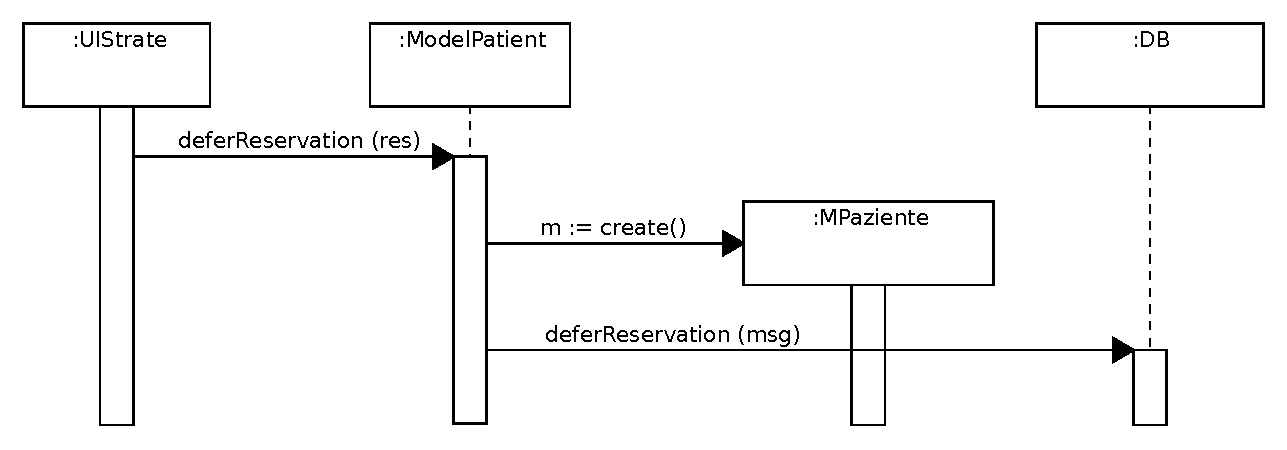
\includegraphics[scale=0.5]{svgs2/p_deferReservation}}\\
   \subfloat[][\emph{fetchReport}.]{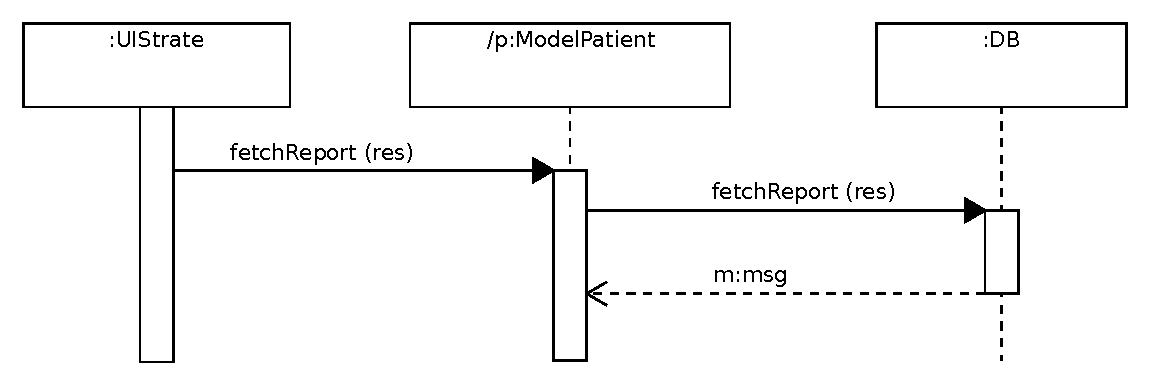
\includegraphics[scale=0.5]{svgs2/p_fetchReport}}\\
   \subfloat[][\emph{login}.]{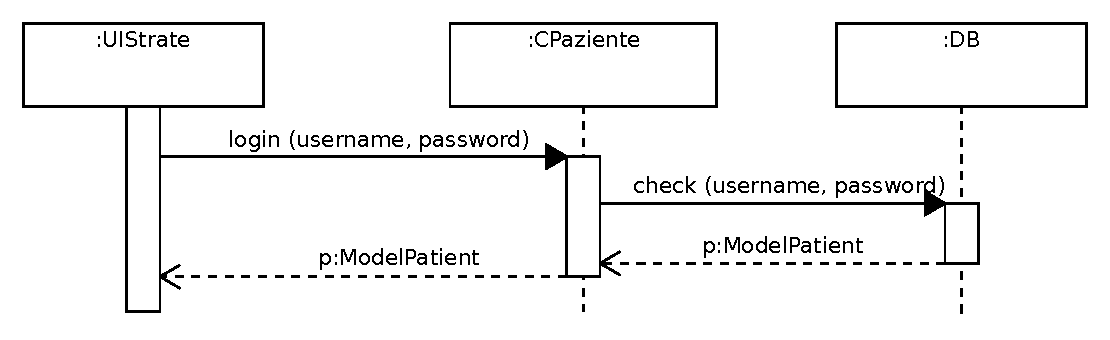
\includegraphics[scale=0.5]{svgs2/p_login}}\\
   \subfloat[][\emph{printOnSupport}.]{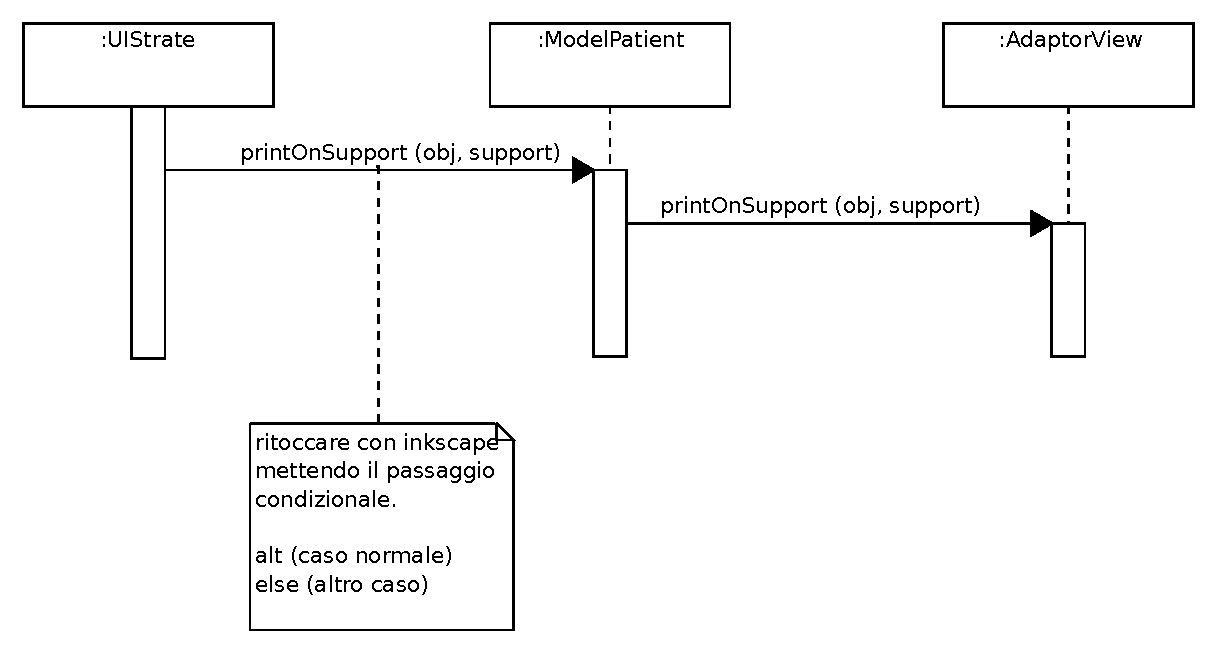
\includegraphics[scale=0.5]{svgs2/p_printOnSupport}}
 \caption{\emph{Use Case Realization for Guest's view (1)}}
\end{figure}

\begin{description}

\item[bindTutorForPatient]

Si utilizza \textbf{Creator}: la responsabilità di associare il tutore al 
paziente è delegata a \texttt{CPaziente}.
Questa operazione viene effettuata solamente all'atto della registrazione, nel 
caso specifico in cui il paziente sia riconosciuto come minorenne. La classe 
\texttt{CPaziente} ha la responsabilità di creare istanze valide di pazienti, ragion
 per cui è sempre essa che prima verifica la fattibilità interpellando il database.
 Naturalemente con la bindTutorForPatient non vengono creati il pazienti minorenni.
 
\item[deferReservation]

Si utilizza \textbf{Information Expert}: la responsabilità di creare il messaggio 
per l'amministratore è delegata alla classe \texttt{ModelPatient}.
Questa operazione e la \texttt{retireReservation} sono quasi identiche: ciò 
che cambia sarà solamente la tipologia del messaggio inviato all'amministratore.
Come già detto precedentemente, si presuppone che l'implementazione della classe 
\texttt{Messaggio} contenga un campo per la discriminazione delle categorie di messaggi.
Non è stata modellata l'eliminazione della prenotazione  in questo stadio,
poiché la gestione delle prenotazioni è esclusivamente dell'amministratore. Quanto
appena detto non esclude la possibilità che l'implementazione finale elimini già 
in questa fase la prenotazione, pur fornendo nel messaggio i dati necessari a 
ricreare la nuova prenotazione.

\item[fetchReport]

Vedi \texttt{fetchReport}. Nel caso specifico \texttt{ModelPatient} non ha bisogno di 
parametri: infatti è sufficiente fornire al DB l'identificativo interno del 
paziente corrente per ottenere tutte le prenotazioni. Si utilizza \textbf{High Cohesion}: 
di fatti a DB viene affidata la responsabilità di prelevare anche le informazioni per il paziente.

\item[login]

Si utilizza \textbf{Information Expert}: La responsabilità di controllare le 
credenziali del paziente è delegata a \texttt{CPaziente}.
Quando l'utente deve ancora autenticarsi, si troverà in uno stato non ancora 
definito, come ospite del sistema. In caso di successo ciò che viene restituito 
sono tutte le informazioni che accertano il paziente nel sistema, per questo ad 
ogni login viene "creato" il paziente verificato. 


\item[printOnSupport]

In questo caso il metodo di stampa vero e proprio dipenderà dal supporto scelto. 
Data la varietà di supporti una scelta vantaggiosa è l'utilizzo di un Facade. 
In questo modo la scalabilità \textit{in the many} richiederà solo l'utilizzo della
classe appropriata per la visualizzazione del contenuto finale.
Si fa ricorso di \textbf{Polymorphism}: di fatti, in base al supporto utilizzato
per effettuare la ``stampa'', \texttt{ViewSupport} avrà poi la responsabilità di 
decidere su quale supporto stampare.

\begin{figure}[!thp]
 \centering
   \subfloat[][\emph{registerNewPatient}.]{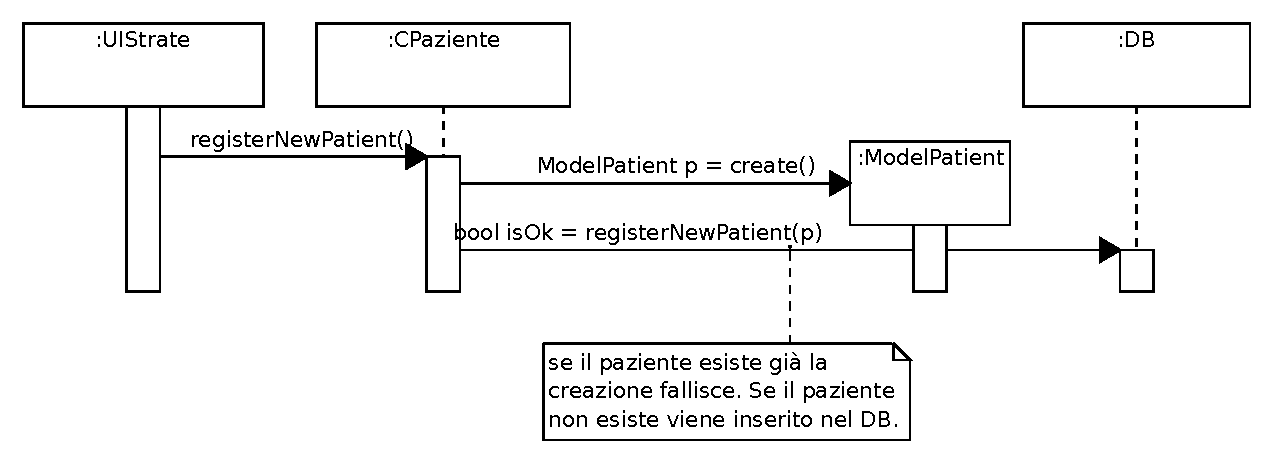
\includegraphics[scale=0.5]{svgs2/p_registerNewPatient}}\\
   \subfloat[][\emph{registerNewPatientFromTutor}.]{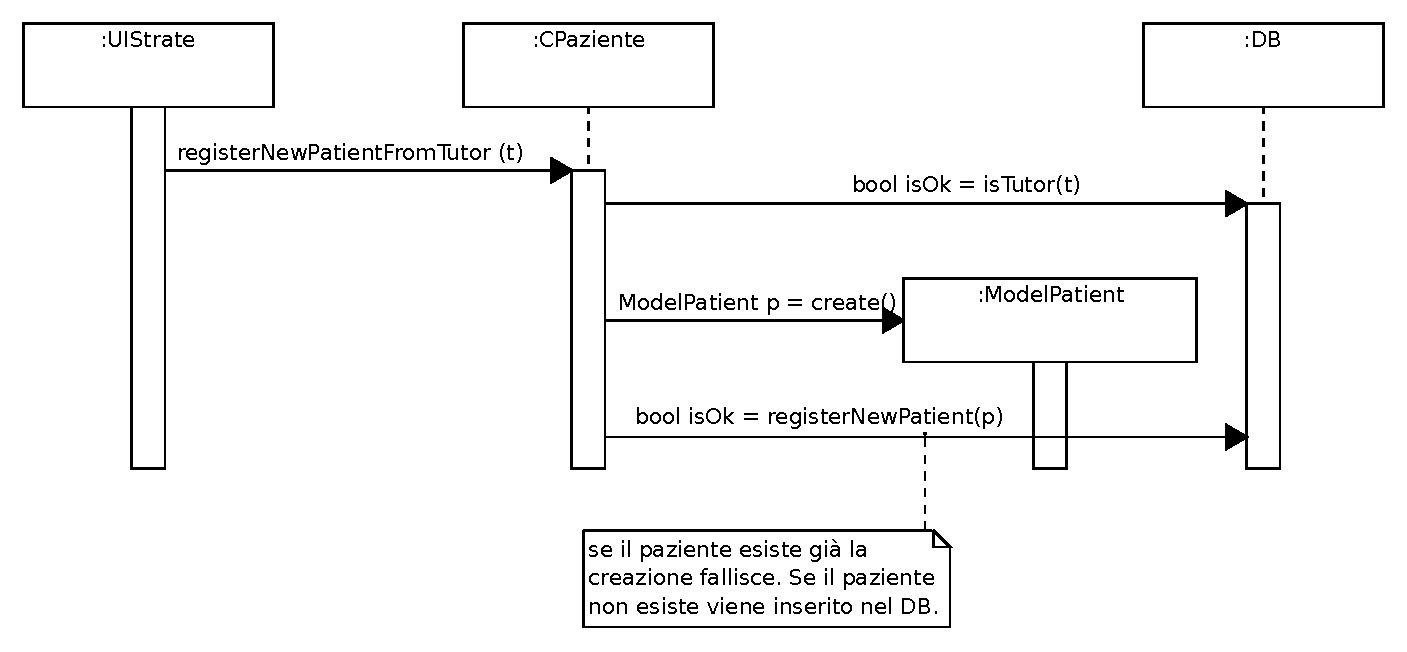
\includegraphics[scale=0.5]{svgs2/p_registerNewPatientFromTutor}}\\
   \subfloat[][\emph{reserveVisit}.]{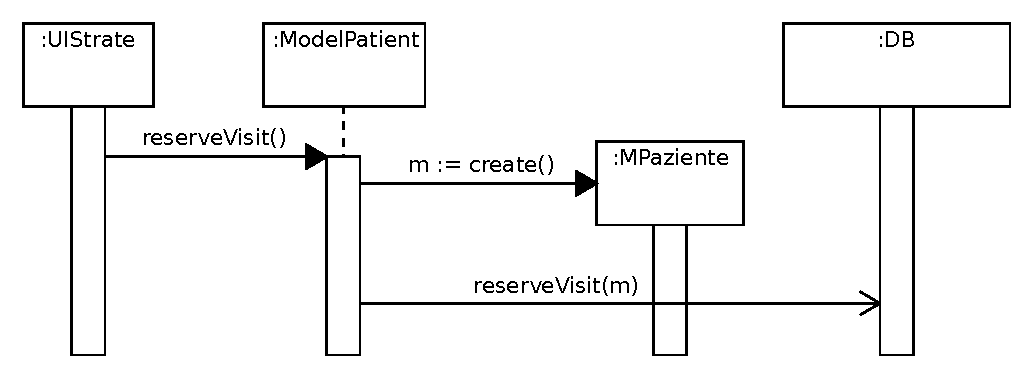
\includegraphics[scale=0.5]{svgs2/p_reserveVisit}}\\
   \subfloat[][\emph{login}.]{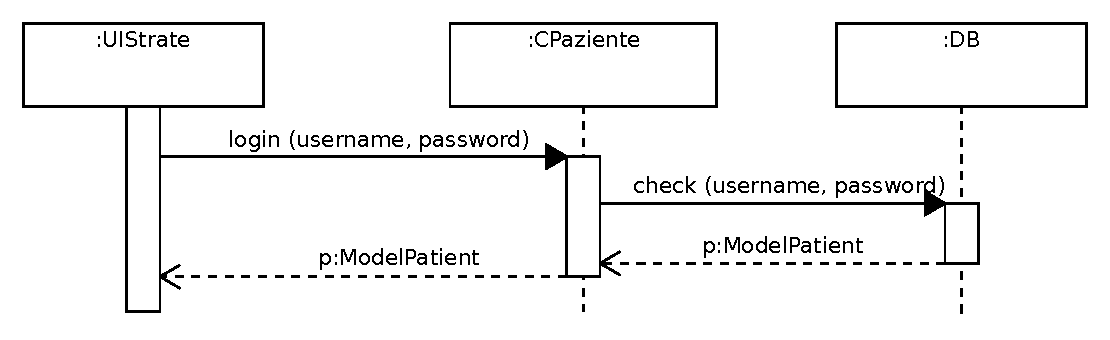
\includegraphics[scale=0.5]{svgs2/p_login}}\\
   \subfloat[][\emph{tutorCredentials}.]{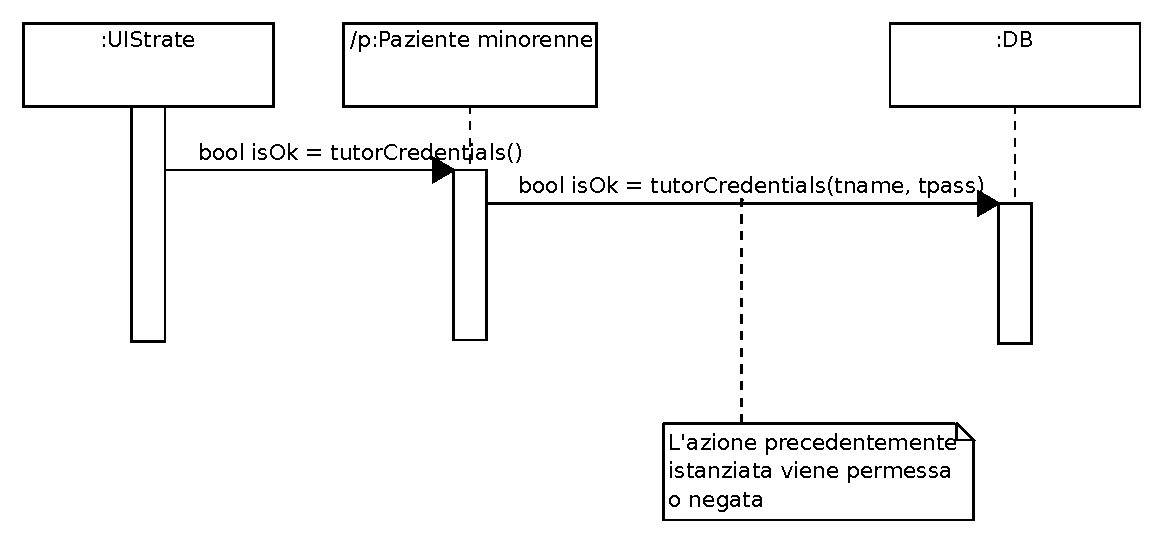
\includegraphics[scale=0.5]{svgs2/p_tutorCredentials}}
 \caption{\emph{Use Case Realization for Guest's view (2)}}
\end{figure}
\begin{figure}[!thp]
	\centering
	\subfloat[][\emph{retireReservation}.]{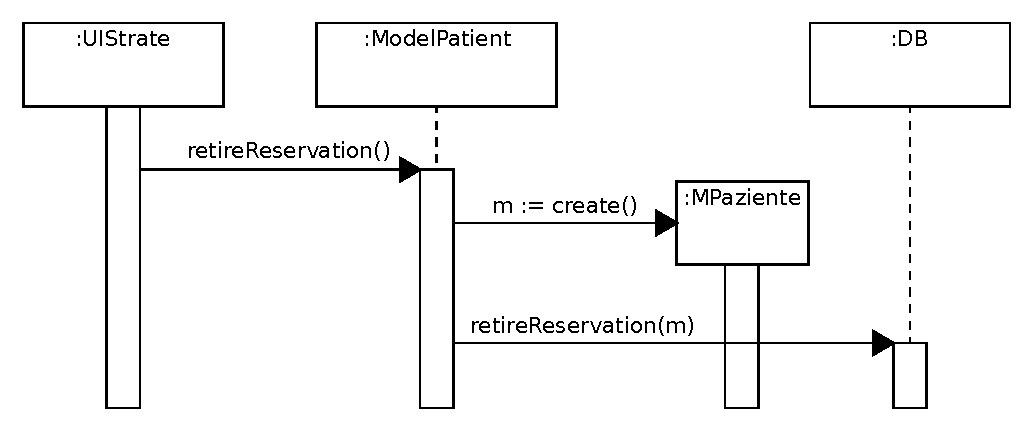
\includegraphics[scale=0.5]{svgs2/p_retireReservation}}\\
	\subfloat[][\emph{registerTutor}.]{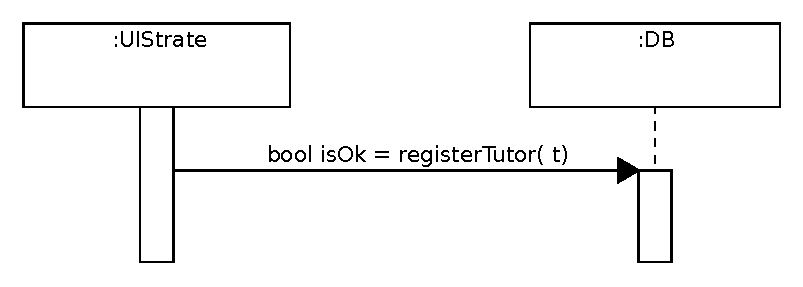
\includegraphics[scale=0.5]{svgs2/p_registerTutor}}\\
	\caption{\emph{Use Case Realization for Guest's view (3)}}
\end{figure}

\item[registerNewPatient]

Si utilizza \textbf{Creator}: di fatti questa la classe che ha la responsabilità 
di creare un nuovo paziente è \texttt{CPaziente}.
In questo caso può si supporre che i dati passati al creatore della classe 
paziente siano validi ( perché vi sono stati controllati precedentemente). 
Si ritiene necessario attribuire alla classe \texttt{CPaziente} anche questa
 responsabilità, in quanto è responsabile della corretta istanziazione delle 
 classi \textit{Paziente}. L'azione di registrazione potrebbe quindi fallire sia in 
 seguito ad un valore non accettabile dal creatore, sia in seguito ad una doppia
 registrazione dell'utente. Non è infatti possibile che lo stesso paziente possa
 essere stato registrato 2 volte.

\item[registerNewPatientFromTutor]

Vedi \texttt{registerNewPatient}. Nel caso specifico anziché costruire il nuovo 
paziente attraverso i dati regolari, viene fornita la possibilità di specificare 
le credenziali di un tutore per registrare il paziente.

\item[reserveVisit]

Si può fare un discorso analogo a quanto fatto per \texttt{deferReservation}. Nel 
caso specifico viene fatta la richiesta di visita, quindi il paziente aspetterà 
una qualche notifica da parte dell'amministratore.

\item[tutorCredentials]

Si utilizza \textbf{Information Expert}: la classe che si occupa di controllare le 
credenziali del paziente è \textit{Paziente minorenne}
Questa caso coinvolge almeno le azioni di registrazione, il login, richiesta di 
prenotazione/annullamento/posticipo di una visita, da parte dell'utente minorenne.


\end{description}


